%2083
\newpage
\section{プログラミングの応用}

\subsection{サンプルフォルダを準備しよう}

上にあるバーのアイコンからファイルマネージャーを開いてみましょう。

\begin{figure}[H]
    \begin{center}
      
\includegraphics[keepaspectratio,width=5.898cm,height=1.242cm]{text04-img/text02-img001.png}
      \caption{ファイルマネージャーを開くアイコン}
    \end{center}
    \label{fig:prog_menu}
\end{figure}

これからHSPで使うことのできるサンプルプログラムをコピーしてもらいます。「/home/ユーザー名」のフォルダに、「sample」フォルダをコピーすることから始めます。

まず、「/usr/local/share/OpenHSP」という場所を開いてみましょう。

この中に、「sample」という名前のフォルダがあります。これから、この「sample」というフォルダを自分の作業フォルダにコピーします。

「sample」という名前のフォルダ上でマウスの右クリックを押して「コピー」を選んでください。


\begin{figure}[H]
    \begin{center}
      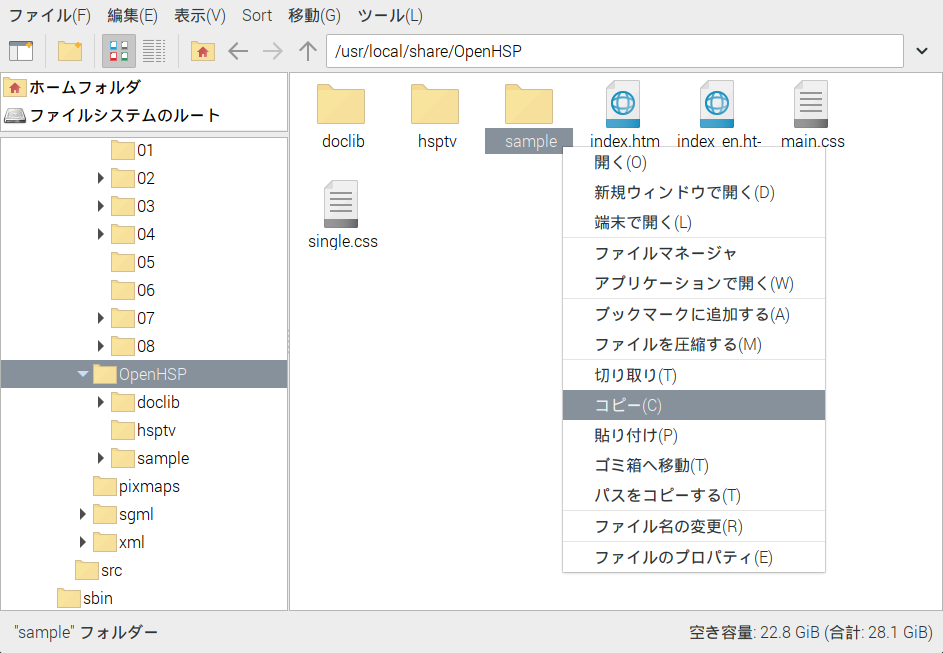
\includegraphics[keepaspectratio,width=11.232cm,height=8.424cm]{text04-img/s_ome04e.png}
      \caption{sampleフォルダでコピーを選ぶところ}
    \end{center}
    \label{fig:prog_menu}
\end{figure}

この後、コピーしたい場所を選びます。コピー先の場所は、「/home/ユーザー名」のフォルダになります。

コピー先の場所を開いたら、何もない場所でマウスの右クリックを押して「貼り付け」を選んでください。

これで先ほどの「/usr/local/share/OpenHSP/sample」フォルダが、「/home/ユーザー名/sample」にコピーされます。

ファイルには、さまざまなプログラムとデータが入っています。

すべてのファイルを紹介できませんが、興味がある人は時間がある時に実際に読み込んで動かしてみましょう。

%2146


